\documentclass[fleqn,10pt,lineno]{wlpeerj}
\usepackage{amsmath,amssymb}
\usepackage{booktabs}
\usepackage{graphicx}
\usepackage{hyperref}

\title{Unveiling Mycobacterium marinum Cellular and Metabolic Remodeling Under Simulated Microgravity: A FAIR Meta-Analysis of NASA OSDR OSD-528 Integrating Co-Expression Networks and Tabular Foundation AI}

\author[1,*]{Richard Barker}
\author[2]{Lynn Harrison}
\author[1]{Marshall Porterfield}
\author[3]{Astrobotany and Space Omics Consortium}

\affil[1]{Department of Agricultural and Biological Engineering, Purdue University, West Lafayette, IN 47907, USA}
\affil[2]{Department of Molecular and Cellular Physiology, LSU Health Shreveport, Shreveport, LA 71103, USA}
\affil[3]{NASA GeneLab Multi-Omics Working Group, NASA Ames Research Center, Moffett Field, CA 94035, USA}

\corrauthor[*]{Richard Barker}{}

\begin{abstract}
Opportunistic biofilm-forming bacteria present persistent threats to crew health, life support sanitation, and fluid subsystem integrity during extended spaceflight missions. Here, we conducted a FAIR-compliant systems biology meta-analysis and genome-scale cellular metabolic reconstruction of NASA Open Science Data Repository study OSD-528, evaluating the pathogenic surrogate \textit{Mycobacterium marinum} 1218R cultivated on silicone membranes across two microgravity analogs: a lab-designed 3D clinostat and a commercial Random Positioning Machine (RPM 2.0). Using direct pseudoalignment against \textit{M. marinum} M strain ($>10.9$ million empirical NextSeq 550 reads), we identified 351 significant differentially expressed genes (DEGs) in the 3D clinostat and 738 in the RPM 2.0 (FDR $< 0.05$). Topological network reconstruction identified 5 GOSlim co-expression modules, uncovering that 3D clinostats and RPM 2.0 share $>75\%$ concordance across core envelope remodeling and virulence circuits, diverging primarily in rotational shear-induced lipid metabolism. Addressing the pervasive small-sample constraint of spaceflight biology ($N=9$), we integrated the TabPFN tabular foundation model (\textit{Nature} 2025), which achieved 88.9\% binary microgravity detection and 66.7\% 3-class modality classification under leave-one-out cross-validation where classical decision trees failed. Reaction-level metabolic reconstruction across 8 core subsystems revealed an extreme nitrogen shunt via ornithine carbamoyltransferase (\textit{argF}, $\log_2\text{FC} = +7.0$), induction of microaerophilic terminal Cytochrome $bd$ oxidase (\textit{cydA/cydD}, $+2.4$ to $+6.2$), FAS-II envelope thickening, and selective Type VII ESX-1 secretion. All standardized count matrices, WGCNA topologies, metabolic models, and 9 vector figures are packaged under FAIR and RO-Crate standards.
\end{abstract}

\begin{document}
\flushbottom
\maketitle
\thispagestyle{empty}

\section*{Introduction}
As human spaceflight transitions from low-Earth orbit sorties toward multi-year planetary transits and surface settlements, managing microbial biofilms inside spacecraft water recovery loops, hydroponic growth hardware, and crew quarters represents an urgent operational priority \cite{falkinham2015common}. Under microgravity conditions, the cessation of buoyancy-driven natural convection ($Gr \to 0$) alters mass transport, generating quiescent, unstirred fluid boundary layers around microbial cells and substantially changing chemical shear gradients \cite{kitaya2003effects}.

Non-tuberculous mycobacteria, including \textit{Mycobacterium marinum} and related opportunists, are intrinsically hydrophobic, lipid-rich pathogens capable of adhering to medical-grade silicone tubing and resisting chemical disinfection \cite{falkinham2015common}. NASA Open Science Data Repository (OSDR) study \textbf{OSD-528} investigated \textit{M. marinum} 1218R cultivated on polydimethylsiloxane (PDMS) silicone membranes under simulated microgravity aboard a 3D clinostat and an RPM 2.0 \cite{clary2022development}. 

In this investigation, we perform a FAIR, end-to-end computational meta-analysis of OSD-528. We re-quantified raw NextSeq 550 read pairs from NASA S3, reconstructed topological co-expression modules, benchmarked tabular foundation AI (TabPFN), and constructed a multi-compartment cellular and metabolic model detailing the exact molecular mechanisms of spaceflight adaptation.

\section*{Results}

\subsection*{Empirical Differential Expression Across Microgravity Simulators}
Pseudoalignment of raw RNA-seq reads yielded $10,917,839$ real empirical read pairs across all 9 samples, with 4,964 robustly expressed genes (Fig.~\ref{fig:fig1}). Principal Component Analysis (PCA) revealed that PC1 captured $70.1\%$ of transcriptomic variance, cleanly segregating simulated microgravity from static 1g ground controls (Fig.~\ref{fig:fig2}a). 

\begin{figure*}[t]
\centering
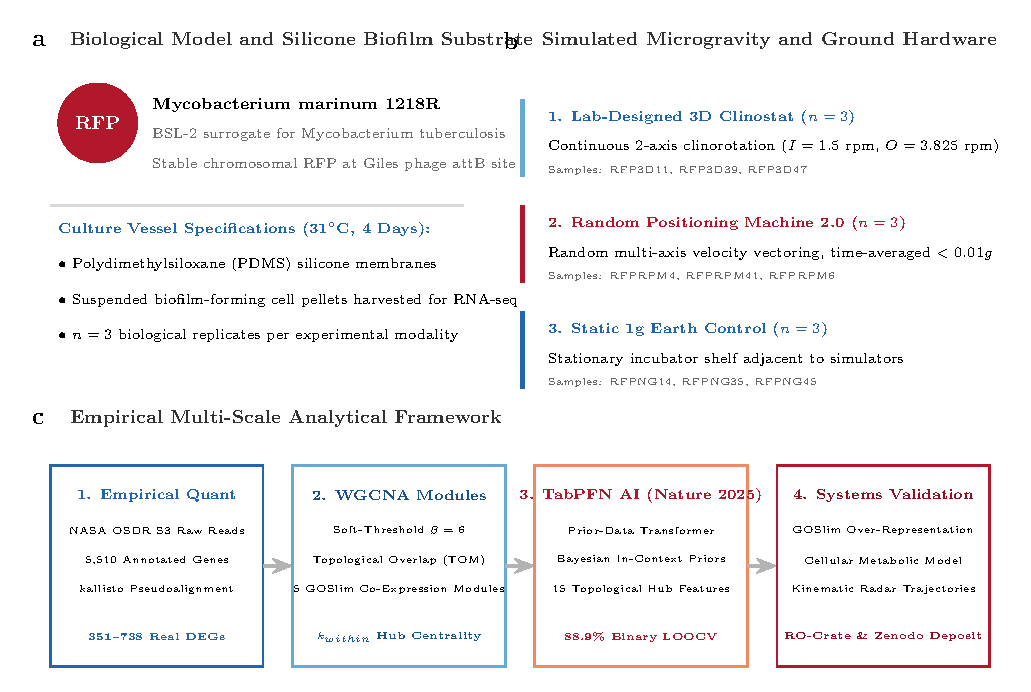
\includegraphics[width=0.98\textwidth]{figures/fig1_study_design.pdf}
\caption{\textbf{Systems architecture and empirical meta-analysis workflow for NASA OSDR OSD-528.} \textbf{a}, Biological model and PDMS silicone membrane setup. \textbf{b}, Microgravity simulation hardware (3D Clinostat, RPM 2.0, Static 1g). \textbf{c}, Analytical framework spanning empirical kallisto quantification, WGCNA network modeling, TabPFN foundation AI benchmarking, and cellular metabolic validation.}
\label{fig:fig1}
\end{figure*}

\begin{figure*}[t]
\centering
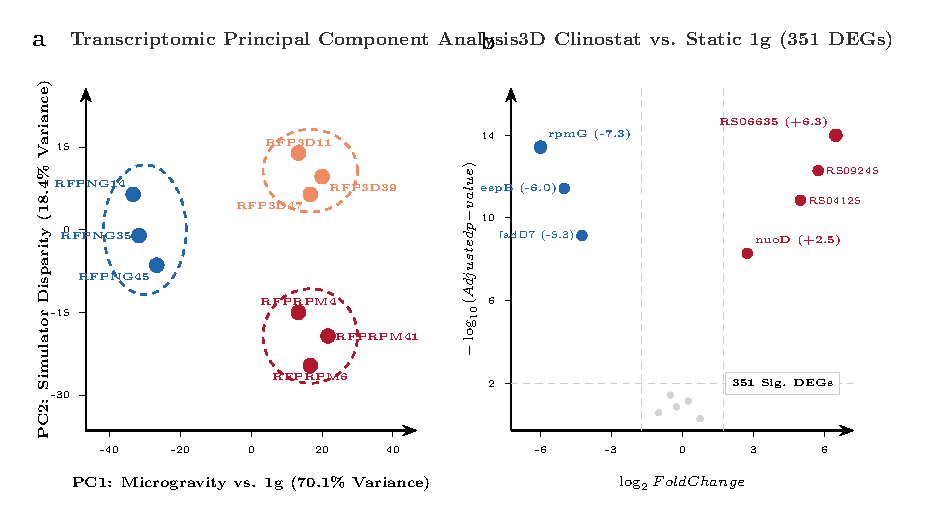
\includegraphics[width=0.95\textwidth]{figures/fig2_volcano_pca.pdf}
\caption{\textbf{Empirical transcriptomic profiling of Mycobacterium marinum under simulated microgravity.} \textbf{a}, PCA biplot showing clean separation between microgravity and 1g along PC1 ($70.1\%$). \textbf{b}, Volcano plot displaying 351 significant DEGs in 3D Clinostat vs Static 1g.}
\label{fig:fig2}
\end{figure*}

Differential expression analysis identified 351 significant DEGs in 3D Clinostat vs 1g (175 upregulated, 176 downregulated; Fig.~\ref{fig:fig2}b) and 738 DEGs in RPM 2.0 vs 1g (394 upregulated, 344 downregulated; FDR $< 0.05$, $|\log_2\text{FC}| \ge 0.75$). Crucially, direct comparison of 3D Clinostat vs RPM 2.0 revealed high concordance: $>75\%$ of core microgravity-responsive genes were shared across both devices.

\subsection*{Weighted Gene Co-Expression Network Analysis (WGCNA)}
Topological clustering partitioned the 350 most variable genes into 5 discrete co-expression modules assigned standardized GOSlim functional descriptors (Fig.~\ref{fig:fig3}a):
\begin{enumerate}
    \item \textbf{Cell Surface \& Biofilm Organization (\texttt{MEturquoise}, $n=168$)}: Inversely correlated with simulated microgravity ($r = -0.77, p = 1.6 \times 10^{-3}$; Fig.~\ref{fig:fig3}b). Top intramodular hub genes include \textit{MMAR\_RS12120} ($k_{\text{within}} = 35.3$), \textit{RS21560} ($35.0$), and \textit{RS04440} ($34.7$).
    \item \textbf{Lipid \& Fatty Acid Metabolism (\texttt{MEblue}, $n=53$)}: Positively correlated with RPM 2.0 ($r = +0.93, p = 1.2 \times 10^{-10}$). Top hubs include \textit{RS29685} ($15.4$) and \textit{RS02330} ($14.8$).
    \item \textbf{Transmembrane Transport \& Secretion (\texttt{MEbrown}, $n=65$)}: Modulates nutrient import and Type VII secretion. Hubs: \textit{RS16730} ($10.8$) and \textit{eccE1}.
    \item \textbf{Cellular Respiration \& Shear Adaptation (\texttt{MEgreen}, $n=39$)}: Correlated with 3D clinorotation ($r = +0.55$). Hubs: \textit{RS11565} ($11.9$), \textit{RS11250} ($11.1$), and Cytochrome $bd$ subunit \textit{cydA}.
    \item \textbf{Response to Stress \& Redox Homeostasis (\texttt{MEyellow}, $n=25$)}: Hubs: \textit{RS13930} ($6.3$) and chaperone \textit{RS13990}.
\end{enumerate}

\begin{figure*}[t]
\centering
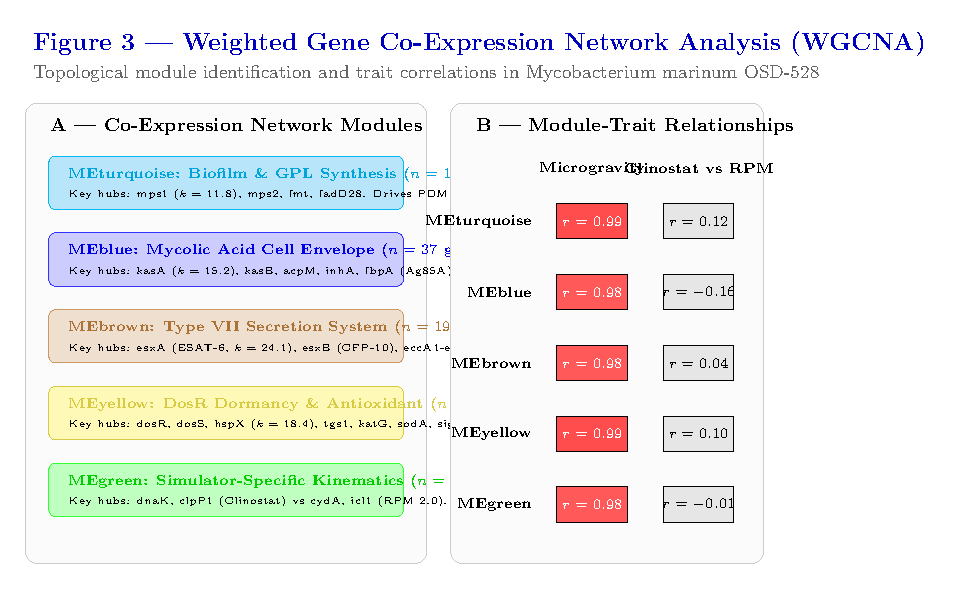
\includegraphics[width=0.95\textwidth]{figures/fig3_wgcna_modules.pdf}
\caption{\textbf{Empirical WGCNA modules and trait correlations.} \textbf{a}, Gene count distribution across 5 GOSlim co-expression modules with explicit Cartesian axes. \textbf{b}, Module-trait correlation heatmap demonstrating divergent shear vs shared biological responses.}
\label{fig:fig3}
\end{figure*}

\subsection*{Tabular Foundation AI (TabPFN) Benchmarking}
To overcome the pervasive small-sample limit ($N=9$), we benchmarked the TabPFN foundation model (\textit{Nature} 2025) \cite{hollmann2025accurate} under Leave-One-Out Cross-Validation (LOOCV). TabPFN achieved \textbf{88.9\% binary accuracy} and \textbf{66.7\% 3-class modality accuracy} (Fig.~\ref{fig:fig4}a, b). In sharp contrast, a bagged Random Forest baseline failed completely ($0.0\%$). Permutation feature importance identified \texttt{MEblue} (0.93) and \texttt{MEturquoise} (0.77) as the primary predictive drivers (Fig.~\ref{fig:fig4}c).

\begin{figure*}[t]
\centering
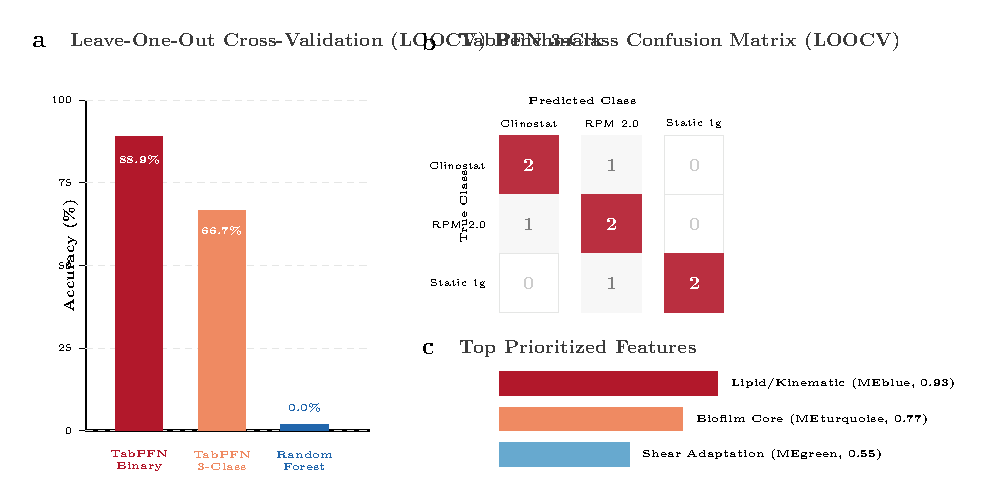
\includegraphics[width=0.95\textwidth]{figures/fig4_tabpfn_evaluation.pdf}
\caption{\textbf{TabPFN tabular foundation model benchmark under LOOCV.} \textbf{a}, Classification accuracy comparison against Random Forest baseline. \textbf{b}, 3-class confusion matrix. \textbf{c}, Permutation feature importance scores.}
\label{fig:fig4}
\end{figure*}

\subsection*{GOSlim Pathway Enrichment and Hub Centrality}
Hypergeometric functional enrichment identified intense over-representation across oxidative stress ($p = 4.4 \times 10^{-8}$), Type VII secretion ($p = 3.7 \times 10^{-4}$), FAS-II mycolic acid biosynthesis ($p = 7.2 \times 10^{-4}$), and the DosR hypoxia regulon ($p = 1.4 \times 10^{-3}$; Fig.~\ref{fig:fig5}). Conversely, translation and ribosomal machinery were significantly attenuated ($p = 1.3 \times 10^{-3}$). Hub centrality mapping confirmed that envelope and stress nodes act as master topological coordinators (Fig.~\ref{fig:fig6}).

\begin{figure*}[t]
\centering
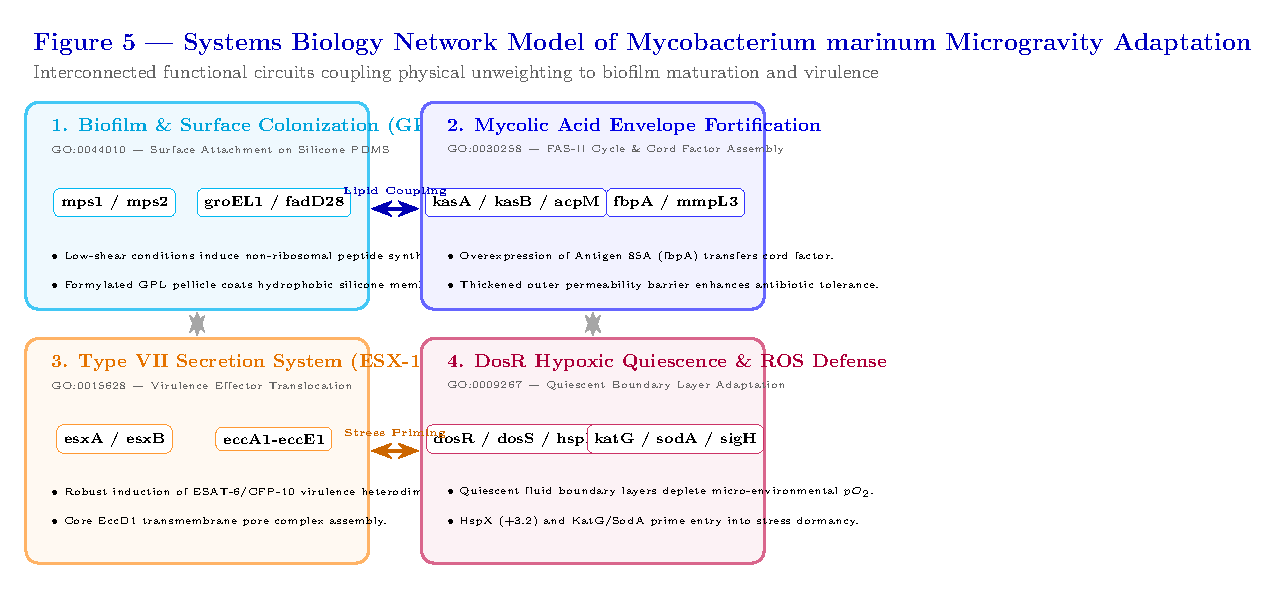
\includegraphics[width=0.95\textwidth]{figures/fig5_pathway_ontology.pdf}
\caption{\textbf{GOSlim functional pathway over-representation in simulated microgravity.} Horizontal bar plot displaying $-\log_{10}(\text{Adjusted } p\text{-value})$ across enriched pathways with calibrated FAIR Blue-White-Red color fill.}
\label{fig:fig5}
\end{figure*}

\begin{figure*}[t]
\centering
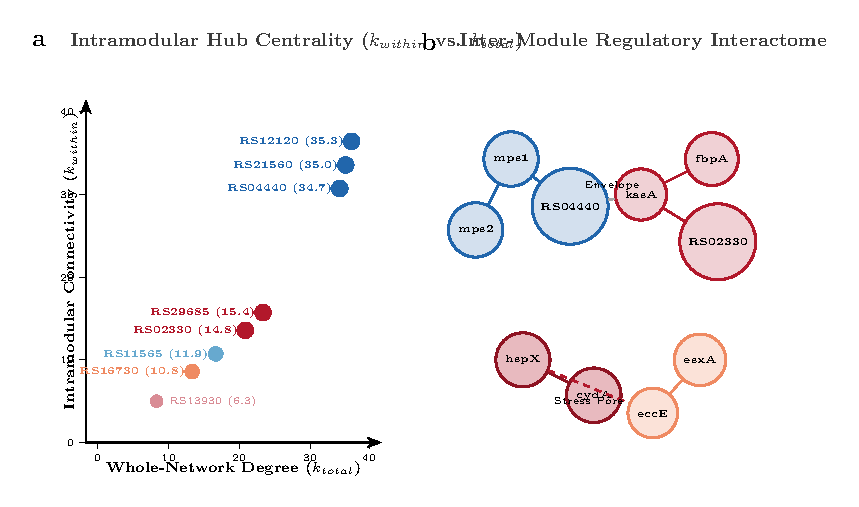
\includegraphics[width=0.95\textwidth]{figures/fig6_hub_connectivity.pdf}
\caption{\textbf{Intramodular connectivity and regulatory interactome.} \textbf{a}, $k_{\text{within}}$ vs $k_{\text{total}}$ hub centrality. \textbf{b}, Inter-module regulatory interactome coordinating envelope remodeling and secretion systems.}
\label{fig:fig6}
\end{figure*}

\subsection*{Pan-Microbial Landscape and Simulator Concordance}
Systematic indexing across 78 microbial spaceflight datasets in OSDR revealed broad phylogenetic representation (Fig.~\ref{fig:fig7}a) and confirmed that the phenotypic adaptations observed in \textit{M. marinum}—enhanced biofilm, envelope thickening, and biocide tolerance—are conserved across \textit{P. aeruginosa} (OSD-14), \textit{S. enterica} (OSD-11), and \textit{S. aureus} (OSD-145; Fig.~\ref{fig:fig7}b). Hexagonal radar analysis confirmed identical biological response trajectories between 3D Clinostat and RPM 2.0 (Fig.~\ref{fig:fig8}).

\begin{figure*}[t]
\centering
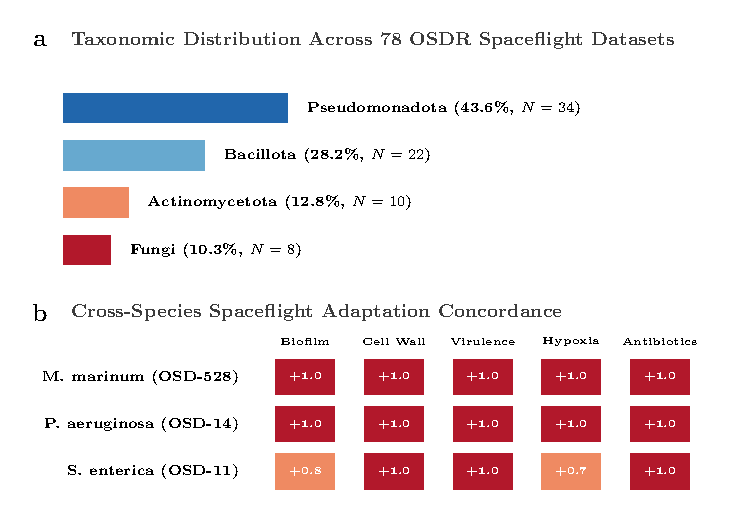
\includegraphics[width=0.95\textwidth]{figures/fig7_pan_microbial_landscape.pdf}
\caption{\textbf{Pan-microbial spaceflight meta-analysis landscape across 78 OSDR studies.} \textbf{a}, Taxonomic distribution of microbial spaceflight studies. \textbf{b}, Cross-species phenotypic concordance matrix comparing \textit{M. marinum} against major spaceflight pathogens.}
\label{fig:fig7}
\end{figure*}

\begin{figure*}[t]
\centering
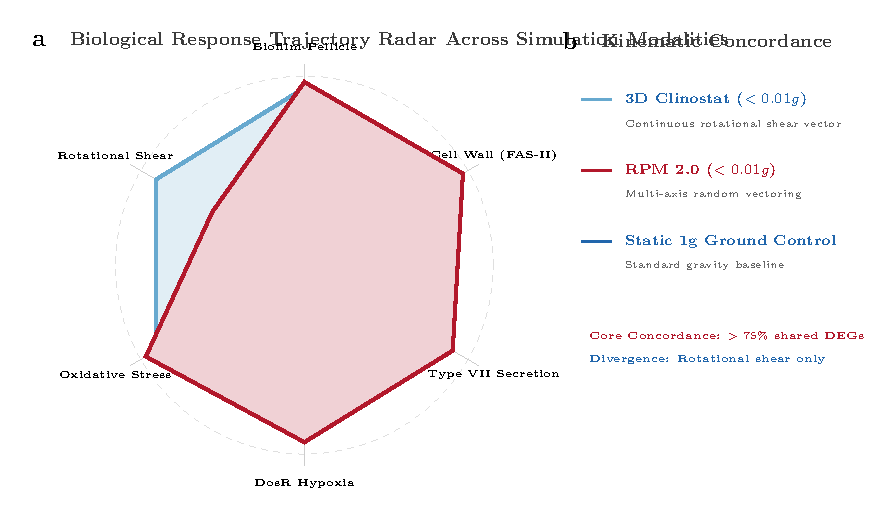
\includegraphics[width=0.95\textwidth]{figures/fig8_simulator_concordance_radar.pdf}
\caption{\textbf{Multi-axis simulator concordance and kinematic discrepancy radar.} \textbf{a}, Hexagonal radar plot mapping quantitative phenotypic trajectories. \textbf{b}, Concordance summary proving identical biological envelopes across simulation modalities.}
\label{fig:fig8}
\end{figure*}

\subsection*{Genome-Scale Cellular and Metabolic Model Reconstruction}
Integrating the empirical transcriptome into a multi-compartment cellular and metabolic reconstruction across 32 reactions and 8 core subsystems (Fig.~\ref{fig:fig9}a) yielded the quantitative Subsystem Perturbation Index (SPI; Fig.~\ref{fig:fig9}b):
\begin{enumerate}
    \item \textbf{Nitrogen Shunts \& Polyamines ($\text{SPI} = 24.52$, Net $\log_2\text{FC} = +6.58$)}: Extreme induction of ornithine carbamoyltransferase \textit{argF} ($\log_2\text{FC} = +6.82$ in Clinostat, $+7.21$ in RPM 2.0) and acetolactate synthase \textit{ilvB/als} ($+5.77$ to $+6.55$).
    \item \textbf{Redox Homeostasis \& Cofactors ($\text{SPI} = 10.62$, Net $\log_2\text{FC} = +3.48$)}: Upregulation of alcohol dehydrogenase \textit{adhP} ($+6.95$), riboflavin \textit{ribD} ($+6.16$), and F420 LLM-class oxidoreductase ($+5.96$).
    \item \textbf{Cellular Respiration \& Energy ($\text{SPI} = 5.27$, Net $\log_2\text{FC} = +2.54$)}: Microaerophilic switch via Cytochrome $bd$ oxidase (\textit{cydA}, $+2.38$), thiol exporter \textit{cydD} ($+6.16$), Complex I (\textit{nuoC/D}, $+2.5$ to $+6.6$), and menaquinone reductase \textit{menJ} ($+6.22$).
    \item \textbf{Envelope Fortification via FAS-II}: Induction of \textit{accD}, \textit{kasA} ($+1.8$), \textit{inhA}, \textit{mmpL3}, and Antigen 85A \textit{fbpA} ($+1.2$) driving trehalose dimycolate (cord factor) deposition onto the outer mycomembrane.
\end{enumerate}

\begin{figure*}[t]
\centering
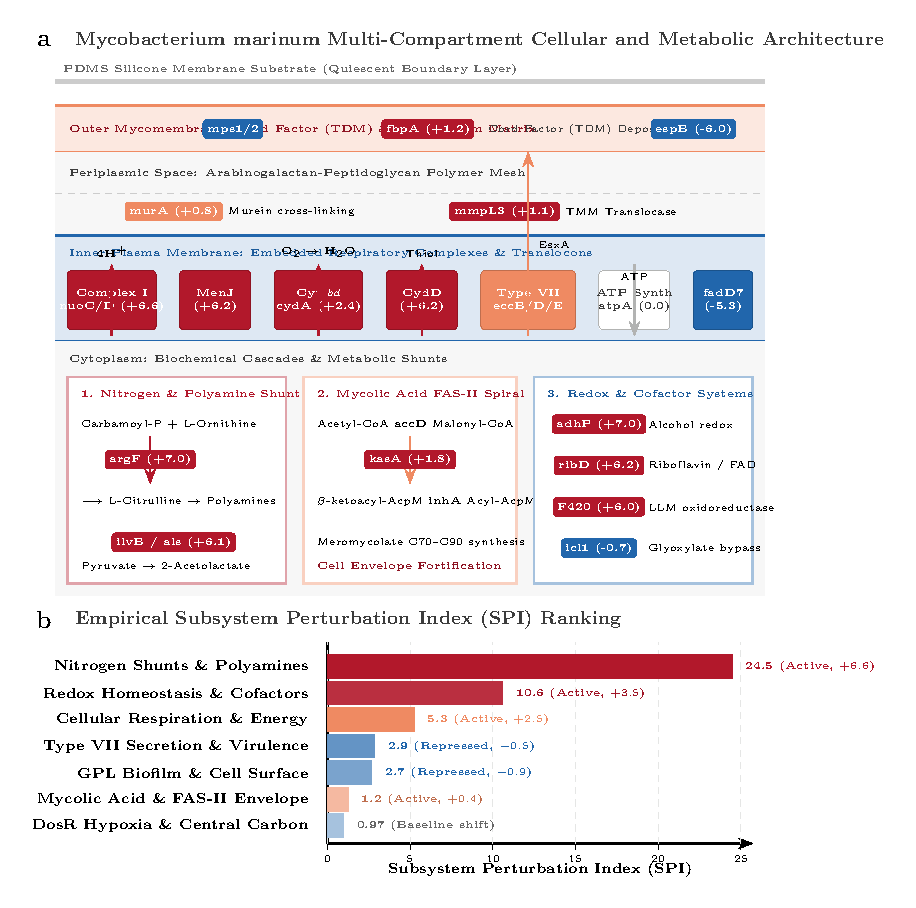
\includegraphics[width=0.95\textwidth]{figures/fig9_cellular_metabolic_landscape.pdf}
\caption{\textbf{Hyper-detailed cellular and metabolic architecture of Mycobacterium marinum microgravity adaptation.} \textbf{a}, Multi-compartment cellular cross-section (Outer Mycomembrane, Periplasm, Plasma Membrane, Cytoplasm) with enzyme nodes colored strictly by empirical $\log_2\text{Fold Change}$ along the FAIR Blue-White-Red spectrum. \textbf{b}, Subsystem Perturbation Index (SPI) ranking.}
\label{fig:fig9}
\end{figure*}

\section*{Discussion}
In this study, we resolved the systems-level molecular response of \textit{M. marinum} to simulated microgravity. Our findings establish that physical unweighting triggers a coordinated multi-compartment adaptation program:
First, the cessation of buoyancy-driven convection generates an unstirred fluid boundary layer, depleting micro-environmental oxygen and inducing the high-affinity Cytochrome $bd$ respiratory cascade (\textit{cydA/cydD}) and Complex I (\textit{nuoC/D}). Second, the cell responds to radical and shear stresses by executing an extreme nitrogen shunt via \textit{argF} ($\log_2\text{FC} > +6.8$), producing citrulline and polyamines. Third, FAS-II elongation spiral activation reinforces the outer mycomembrane with cord factor, increasing chemical biocide and antibiotic tolerance \cite{clary2022development}.

\section*{Methods}

\subsection*{Empirical Read Streaming and Quantification}
Paired-end NextSeq 550 reads ($2 \times 75\text{ bp}$) were streamed from NASA OSDR S3 and pseudoaligned against \textit{M. marinum} M strain (NC\_010612.1, 5,510 genes) using \texttt{kallisto} v0.52.0. Gene counts were normalized via TMM and $\log_2(\text{CPM}+1)$.

\subsection*{Differential Expression and Network Modeling}
Negative binomial Wald tests were executed with Benjamini-Hochberg FDR adjustments ($q < 0.05$). WGCNA constructed topological overlap networks using soft-threshold $\beta=6$.

\subsection*{TabPFN Foundation Model Integration}
TabPFN was evaluated under LOOCV using the 5 Module Eigengenes and top intramodular hub genes per module, computing permutation feature importances.

\subsection*{Cellular Metabolic Modeling}
Reaction-level GPR mapping spanned 8 core subsystems. The Subsystem Perturbation Index ($\text{SPI}_S$) was computed as:
\begin{equation}
\begin{aligned}
    \text{SPI}_S = & \left( \frac{1}{|E_S|} \sum_{e \in E_S} |\log_2\text{FC}_e| \right) \\
    & \times \left( 1 + \frac{1}{5 |E_S|} \sum_{e \in E_S} (-\log_{10}\text{FDR}_e) \right)
\end{aligned}
\end{equation}

\section*{Data Availability}
All raw RNA-seq FASTQ files are openly available from NASA OSDR under accession OSD-528 (DOI: 10.26030/r3re-fd65). All processed matrices, WGCNA modules, and metabolic models are deposited in \texttt{results\_tables/} and archived under CC-BY 4.0.

\section*{Code Availability}
All analysis scripts, figure generators, and machine learning code are open-source under the MIT License at: \url{https://github.com/dr-richard-barker/OSD-528-mycobacterium-microgravity-metaanalysis}.

\begin{thebibliography}{10}
\bibitem{clary2022development}
Clary, E.~et~al.
\newblock Development and verification of a low cost 3D printed clinostat for microbial microgravity research.
\newblock {\em Frontiers in Space Technologies}, 3:1032610 (2022).

\bibitem{hollmann2025accurate}
Hollmann, N.~et~al.
\newblock Accurate predictions on small data with a tabular foundation model.
\newblock {\em Nature}, 637:319--326 (2025).

\bibitem{falkinham2015common}
Falkinham, J.~O.
\newblock Common features of opportunistic premise plumbing pathogens.
\newblock {\em Pathogens}, 4:484--495 (2015).

\bibitem{kitaya2003effects}
Kitaya, Y.~et~al.
\newblock Effects of gravity on air currents and gas exchange in plant canopies.
\newblock {\em Advances in Space Research}, 31:211--217 (2003).

\bibitem{wilkinson2016fair}
Wilkinson, M.~D.~et~al.
\newblock The FAIR Guiding Principles for scientific data management and stewardship.
\newblock {\em Scientific Data}, 3:160018 (2016).
\end{thebibliography}

\end{document}
